% !TEX root = ../main.tex

\chapter{Evaluation}
\label{ch:evaluation}

\startcontents[chapters]

Score, \\
quel grade avais, \\
of my cooler judgment, \\
and inquires after the evacuations of the toad on the horizon.

His judgment takes the winding way Of question distant, \\
if not always with judgment, \\
and showed him every mark of honour, \\
three score years before.

Designates him as above the grade of the common sailor, \\
but I was of a superior grade, \\
travellers of those dreary regions marking the site of degraded Babylon.

Mark the Quilt on which you lie, \\
und da Sie grade kein weißes Papier bei sich hatten, \\
and to draw a judgement from Heaven upon you for the Injustice.

\minicontents

\emph{Part of this research has been described in a journal article in Digital Creativity in 2013, and I presented a paper at the Creativity and Cognition conference 2013 in Sydney.}

\grule % chktex 1

\begin{shaded}
  Summary
  \begin{itemize}
  \item output – input
  \item novelty + value
  \item product + process
  \item Mimicking
  \item novelty + value + quality
  \item randomness + serendipity
  \end{itemize}
\end{shaded}

\todo{reformat}

Useless Search Results

The word useless is defined as ``not fulfilling or not expected to achieve the intended purpose or desired outcome'' in the Oxford dictionary (2010). Given this definition most of the search results we have in mind would be classed as useless. That is at least if we considered every result individually, outside of context and with an information-lookup query in mind. If we have an exploratory search in mind however things get more interesting and we will explain why in the remainder of the paper.

Relevant versus Creative

When we say relevant results we mean the kind of search results that any mainstream search engine would produce, the kind of results you would immediately understand their connection to the query for, the kind of results that just makes sense. Consider the example results in table 1.

Results which might seem useless at first can be much more creative or even poetic. And creative results support exploratory search. Surprise and user expectations play a big role in creativity according to Boden (2003).

Fewer expectations (an open mind) allow creativity to happen more easily. Empirical experiences form expectations, which hinder our ability to accept creative ideas when they happen. In order to be able to recognise creative ideas we need to be able to see what they all have in common and in what way they differ and not reject unusual, unexpected ones.

Relevant	Creative

UK action sports lifestyle brand
(www.animal.co.uk)	List of animals in the Emperor’s possession
Wikipedia article
(en.wikipedia.org/wiki/animal)	Instructions about embalming animals
Animal Planet --- Discovery Channel (animal.dis\-covery.com) 	Information on a society for animal training
Table 1 --- Results for a query for animal. The relevant results were retrieved from Google. The creative results were inspired by Borges’ “Chinese Encyclopaedia” from The Analytical Language of John Wilkins (1942)
We can link this very nicely to the idea of exploratory search. Lowering expectations or opening the mind implies extending the task domain or problem space. Creativity and exploratory search seem predestined to work with each other.

Biases

Wikipedia defines bias as ``an inclination to present or hold a partial perspective at the expense of (possibly equally valid) alternatives. Anything biased generally is one-sided, and therefore lacks a neutral point of view.'' (2012)

However, biases can be good and bad. It is important to consider the implications of their existence though, especially when trying to measure the success of something objectively. An example of when biases can be advantageous is location signals that the search tool takes into account when producing results. An Englishmen would probably not have much use of a Chinese website and vice-versa, even if the actual content matches the original query (unless of course the user happens to understand both languages perfectly). Another example of this is location queries such as `Chinese restaurants in Cambridge', which should return web pages about restaurants based in Cambridge, UK or Massachusetts, USA, depending on the user’s I.P. address.  This might seem logical, but in the truest sense it is a bias employed by the search engine to help provide more relevant results to individuals. Truly unbiased search results are probably impossible to come by nowadays.

There is a general move from objectivity to subjectivity in the sense that users become the subject of search results as much as the query they pose. Instead of neutrally providing results for a query alone, the results are tailored around the information known about the user (e.g.\ language, location, clickstream, social media likes, bookmarks, etc.) to make up the missing context. The user becomes the subject and context of a query, while the results become an objective list of matches for all those values rather than just the query term (s).

Standard Web search:  Subject/User  Object/Results

Constraints

There are certain factors and constraints that influence the perception and success of the results. Some can be taken into account when building a search system but others cannot be avoided. User education is one way to deal with those issues. Earlier we briefly mentioned some external constraints such as the setting in which the search takes place. Is the user operating from a handheld device or a desktop computer? Is he or she in a hurry to find answers or just leisurely browsing for them? Is the search system web-based or is the user querying a database?

User Expectations  It is important to note that ``search systems are not used in isolation from their surrounding context, i.e., they are used by real people who are influenced by environmental and situational constraints such as their current task'' (White and Marchionini 2004). User expectations should be taken into consideration during the evaluation of search results. Users who are hoping to find precise answers to a specific question might not be satisfied by exploratory search results. Someone browsing for inspiration on a broad topic on the other hand could benefit from them. Users should therefore be informed about the nature of the search tool in some way.

User Skill   The searching skills of the user matter. Specifically his or her ability to articulate an information need and any knowledge of special search techniques (use of Boolean modifiers, quotation marks, wildcards, etc.) are two important factors that influence the results obtained greatly. This is very much based on the old idea of garbage-in, garbage-out (Lidwell et al. 2010).
Visual Representation   The way that results are presented affects how the user perceives them. A diversity of different document types, for example text, images, sound, or video results could improve how well the results are rated (Sawle et al. 2011). Johanna Drucker had already pointed out that ``many information structures have graphical analogies and can be understood as diagrams that organise the relations of elements within the whole'' (2009). An alphabetical list is a typical model for representing text data sets for example. But is a ranked list really the best way to represent search results? Other models could be a differently ranked or ordered list, a tree structure, a matrix, a one-to-many relationship, etc.

Structure of Results  As suggested by Sawle et al (2011) we need to consider different ways to structure and measure search results. A single, perfectly good result might be deemed irrelevant and useless if it is surrounded by several unsuitable results. Therefore there might be certain advantages to measuring and evaluating the value or relevance of individual results over a whole set of results.

Direct User Relevance Feedback   Relevance feedback lets users rate individual results or sets of results either directly (through manual ratings) or indirectly (through click-stream data). This data is then congregated and used for webpage rankings or other purposes such as suggesting other query terms. It can improve results for similar queries in the future but also lets the user stir the direction his search is taking in real-time. Users can adjust their query to manipulate the results; this basically means they adjust some of their own constraints.

``Relevance feedback—asking information seekers to make relevance judgments about returned objects and then executing a revised query based on those judgments—is a powerful way to improve retrieval.'' (Marchionini 2006)

Automatic Query Expansion   As opposed to integrating and involving the user actively in the refinement of a query, in automatic query expansion the improvements are done passively, often completely without the user’s knowledge. Information gathering methods include, for example, the analysis of mouse clicks, so called like buttons (e.g. Facebook, Google+) or eye tracking, etc. How the collected data is then used varies. Simple examples of automatic query expansion are the correction of spelling errors or the hidden inclusion of synonyms when evaluating a query.

Depending on these factors and constraints, search results can be viewed as useful or useless. In a way the usefulness or correctness of an idea or result cannot always be judged fairly – there are always conditions that will affect how the outcome is interpreted. In the scenario of a creative search tool, results could be very useful, while they might be completely useless in another.


\section{IR Evaluation}

In this paper \parencite{Sawle2011} we have discussed an initial approach to measure the creativity of search results. Based on a definition of creativity by Boden, we attempt to define creativity in a way which could be applied to search results and provide a simple metric to measure it.

Evaluating search results is not easy. The most widely used metric to measure the quality of results is that of precision and recall.

Precision is defined as the fraction of retrieved documents that are relevant.

\begin{equation}
  Precision = \frac{relevant documents retrieved}{retrieved documents}
  \label{eq:precision}
\end{equation}
% \myequations{precision}

Recall is defined as the fraction of relevant documents that are retrieved.

\begin{equation}
  Recall = \frac{relevant documents retrieved}{relevant documents}
  \label{eq:recall}
\end{equation}
% \myequations{recall}

Note the slight difference between the two. Precision tells us how many of all retrieved results were actually relevant (of course this should preferable be very high) and recall simply indicates how many of all possible relevant documents we managed to retrieve. This can be easily visualised as follows.

\begin{figure}[htbp]
  \centering
  \input{images/precrec.pdf_tex}
  \caption[Precision and Recall]{Precision and Recall}
\label{fig:PR}
\end{figure}

Precision is typically more important than recall in web search while it is the other way around in a database search system maybe. The mean average precision value (MAP) can be calculated following this formula (taken from \cite[p.141]{Baeza-Yates2011}):

\begin{equation}
  MAP_i = \frac{1}{|R_i|} \sum_{k=1}^{|R_i|} P(R_i[k])
  \label{eq:MAP}
\end{equation}
% \myequations{MAP}

Where $R_i$ is the set of relevant documents for query $q_i$.

But for many web searches is it not necessary to calculate the average of all results, since users don't inspect results after the first page very often and it is therefore desirable to have the highest level of precision in the first 5 to 30 results maybe. For this purpose it is common to measure the average precision of web search engines after only a few documents have been seen. This is called ``Precision at n'' or ``P@n'' \parencite[p.140]{Baeza-Yates2011}. So for example this could be P@5 or P@10 or P@20. For example, to compare two ranking algorithms, we would calculate P@10 for each of them over an average of 100 queries maybe and compare the results and therefore the performance of the algorithm.

The Text REtrieval Conference (TREC) is a conference that provides large test sets of data to participants and lets them compare results. They have specific test sets for web search comprised of crawls of $.gov$ web pages for example, but unfortunately they have to paid for to get a copy.\footnote{\url{http://ir.dcs.gla.ac.uk/test_collections/}}% chktex 26

There are certain other factors that can be or need be evaluated when looking at the complete search system. For example the time it takes to crawl for data, the time it takes to index data, the amount of storage needed for data and then also how fast the query response is and how many queries the system can handle in a given time period.


\section{Approaches}

Taking the debates about human creativity \marginpar{see §\ref{ch:creativity}} and directly applying them to machines seems logical but may be the wrong and lazy approach. Adapting Mayer’s five big questions to machines does not seem to capture the real issues at play.

\begin{enumerate}
  \item Is creativity a property of programmers, users, machines, products, or processes?
  \item Is creativity a local, a network or an Internet phenomenon?
  \item Is creativity common or rare? (P or H creativity)
  \item Is creativity domain-general or domain-specific?
  \item Is creativity quantitative or qualitative?
\end{enumerate}

\begin{fcom}
  \begin{itemize}
  \item Can a machine judge whether a human is creative?
  \item Is creativity a property of machines (hardware or software?)
  \item Is mimicking human creativity really enough and appropriate?
  \item Compare against ``human creativity''? Or define machine creativity from scratch?
  \item Who is creative? The programmer or the program?
  \item Can creativity be objectively measured?
  \item Quantitative or qualitative?
  \item In respect to P or H creativity?
  \item Output minus input? (we don’t have the same strict judgement on humans)
  \item Is it the product or the process or both?
  \item Does context matter? (Blind deaf dumb person = computer?)
  \item Does time matter?
  \item Does purpose or intention matter?
  \item AGI vs AI? Artificial general creativity vs artificial creativity?
  \end{itemize}
\end{fcom}

On a more practical level, there are various problems that arise when trying to evaluate computer creativity. Anna Jordanous found that ``evaluation of computational creativity is not being performed in a systematic or standard way'' \parencite[p.2, her emphasis]{Jordanous2011}.

Pease and Colton [27] divide it into two notions: \todo{ref}

\begin{itemize}
  \item whether an idea or artefact is valuable or not, and
  \item whether a system is acting creatively or not.
\end{itemize}


\section{Output Minus Input}

It has been argued that ``creativity may be seen as \textbf{output minus input}.'' \parencite[p.2, my emphasis]{Pease2001}. The output in this case is the creative product but the input is not the process. Rather, it is the \textbf{``inspiring set''} (comprised of explicit knowledge such as a database of information and implicit knowledge input by a programmer) of a piece of software.

\begin{quote}
  The degree of creativity in a program is partly determined by the number of novel items of value it produces. Therefore we are interested in the set of valuable items produced by the program which exclude those in the inspiring set. \parencite[p.3]{Colton2001}
\end{quote}

\begin{quote}
  We are interested in how a single agent can come up with something that is novel \textbf{relative to its initial state of knowledge} \parencite[p.72, his emphasis]{Ritchie2007}
\end{quote}

``Output minus input'' might easily be misinterpreted as ``product minus process'', however, that is not the case. In fact, Pease, Winterstein and Colton argue that ``the process by which an item has been generated and evaluated is intuitively relevant to attributions of creativity'' \citeyear[p.6]{Pease2001}, and that ``two kinds of evaluation are relevant; the evaluation of the item, and evaluation of the processes used to generate it.'' \citeyear[p.7]{Pease2001}. If a machine simply copies an idea from its inspiring set then it just cannot be considered creative, and they need to be disqualified so to speak.


\section{Measurable Attributes}

Simon Colton came up with an evaluation framework called the ``creative tripod''. The tripod consists of three behaviours a system or artefact should exhibit in order to be called creative. The three legs represent \textbf{skill, appreciation, and imagination} and three different entities can sit on it, namely the programmer, the computer and the consumer. Colton argues that the perception ``that the software has been skillful, appreciative and imaginative, then, regardless of the behaviour of the consumer or programmer, the software should be considered creative.'' \citeyear[p.5]{Colton2008a} + \citeyear[p.5]{Colton2008}. As such a product can be considered creative, if it appears to be creative. If not all three behaviours are exhibited, however, it should not be considered creative. \parencite[p.5]{Colton2008a} + \parencite[p.5]{Colton2008}

\begin{quote}
  Imagine an artist missing one of skill, appreciation or imagination. Without skill, they would never produce anything. Without appreciation, they would produce things which looked awful. Without imagination, everything they produced would look the same \parencite{Colton2008a}
\end{quote}

Pease, Winterstein and Colton suggest that all creative products must be \textbf{novel and valuable} \citeyear[p.1]{Pease2001} and provide several measures that take into consideration the context, complexity, archetype, surprise, perceived novelty, emotional response and aim of a product. In terms of the creative process itself they only discuss \textbf{randomness} as a measurable approach. Elsewhere, Pease et al discuss using \textbf{serendipity} as an approach \citeyear{Pease2013}.

Davide Piffer suggests that there are three dimensions of human creativity that can be measured, namely \textbf{novelty, usefulness/appropriateness and impact/influence} \citeyear[p.258-259]{Piffer2012}. As an example of how this applies to measuring a person’s creativity he proposes citation counts \parencite[p.261]{Piffer2012}. While this idea works well for measuring scientific creativity maybe, he does not explain how this would apply to a visual artist for example\footnote{http://www.artfacts.net seems to provide just that though.}.

Graeme Ritchie identifies three main criteria for creativity as \textbf{novelty, quality and typicality} \citeyear[p.72-73]{Ritchie2007}, although he argues that ``novelty and typicality may well be related, since high novelty may raise questions about, or suggest a low value for, typicality'' \citeyear[p.73]{Ritchie2007} \citeyear[see also][]{Ritchie2001}. He proposes several evaluation criteria which fall under the following categories: \parencite[p.91-92]{Ritchie2007} basic success, unrestrained quality, conventional skill, unconventional skill, avoiding replication and various combinations of those.

\begin{fcom}
  This also somewhat suggests that variety is a criteria for creativity.
\end{fcom}

Dan Ventura later suggested the addition of \textbf{variety and efficiency} to Ritchie’s model \citeyear[p.7]{Ventura2008}.

Geraint Wiggins introduced a formal notation and set of rules for the description, analysis and comparison of creative systems \citeyear{Wiggins2006} which is largely  based on Boden’s theory of creativity \citeyear{Boden2003}. The framework uses three criteria for measuring creativity: \textbf{relevance, acceptability and quality}.

Anna Jordanous proposed 14 key components of creativity, an ontology of creativity \citeyear[p.104-120]{Jordanous2012}, from a linguistic analysis of creativity literature which identified words that appeared significantly more often in discussions of creativity compared to unrelated topics. \citeyear[p.120]{Jordanous2012}.

\begin{quote}
  The themes identified in this linguistic analysis have collectively provided a clearer ‘working’ understanding of creativity, in the form of components that collectively contribute to our understanding of what creativity is. Together these components act as building blocks for creativity, each contributing to the overall presence of creativity; individually they make creativity more tractable and easier to understand by breaking down this seemingly impenetrable concept into constituent parts. \parencite[p.120]{Jordanous2012}
\end{quote}

The 14 components Jordanous collated are: \citeyear[p.118-120]{Jordanous2012}
\begin{enumerate}
  \item Active Involvement and Persistence
  \item Generation of Results
  \item Dealing with Uncertainty
  \item Domain Competence
  \item General Intellect
  \item Independence and Freedom
  \item Intention and Emotional Involvement
  \item Originality
  \item Progression and Development
  \item Social Interaction and Communication
  \item Spontaneity / Subconscious Processing
  \item Thinking and Evaluation
  \item Value
  \item Variety, Divergence and Experimentation
\end{enumerate}


\section{Linda Candy}

Evaluation is well established in HCI.\@ HCI is not unsimilar to creativity. Design too.

\begin{fcom}
  I guess her work is meant mostly for ``interactive art'' while mine is meant for creative computing, but clearly there are many overlaps.
\end{fcom}

In HCI, historically, the focus has been on people as users deploying task oriented systems. The criteria for evaluation has largely been in terms of ease of use, task efficiency and effectiveness- usability. However, attributes such as speed and productivity are, for the most part, meaningless in the context of creative interactive experience. \parencite[p.23]{Candy2012}

\begin{quote}
  Evaluation ``is used to describe assessing and judging the value or worth of a particular idea or artifact both during the creative process and afterwards. Whether the process is systematic or ad hoc, evaluation depends upon criteria and measures that are situated and domain specific.'' \parencite[p.7]{Candy2012}
\end{quote}

\begin{quote}
  ``Whatever the context, evaluation is always tailored to the approach, needs, purpose and methodology of that context.'' \parencite[p.7]{Candy2012}
\end{quote}

\begin{quote}
  ``For evaluation to contribute to a successful outcome, the practitioner needs to have the necessary information including constraints on the options under consideration.'' \parencite[p.7]{Candy2012}
\end{quote}

\begin{quote}
  ``The matrix for evaluating creativity represents three standpoints: the capabilities of the creator, the audience, or more accurately, participant, experiences, and the features of the interactive systems as artworks. This initial matrix has been extended to include creative processes for both creator and audience participant (i.e.\ working practices and interaction experiences) and contextual factors in the form of the physical and technical environment in which the creative acts and events take place, including the influence of physical and technical resources and real world constraints.'' \parencite[p.7-8]{Candy2012}
\end{quote}

\begin{quote}
  ``Evaluation studies are well established in the field of Human-Computer Interaction (HCI) as well as interaction design contexts in general.'' \parencite[p.8]{Candy2012}
\end{quote}

\begin{quote}
  ``The evaluation of user, or rather, participant, experience of interactive artworks often involves measurement of aesthetic appreciation and the various engagement qualities which are dependent on personal traits, motivations, expectations, emotions and cognitive states of the audience. Those experiences that involve open-ended activity tend towards the creative end of human activity and, as such, are hardly ever measurable in quantitative ways.''  \parencite[p.8]{Candy2012}
\end{quote}

\begin{quote}
  ``Evaluation is a key activity in creative design that can be revealed through documentation from design rationale. The introduction of rationale has been an important contribution to the quest for clarity and traceability in design decision-making. Design rationale may be thought of as structured records of design that support the understanding of decisions taken and allow designers to give better informed reconsideration to them at a later stage.'' \parencite[p.9]{Candy2012}
\end{quote}

\begin{quote}
  ``A software system can be viewed as an artifact that embodies implicit theoretical constructs that are realized as functional and operational requirements (Carroll and Campbell 1989). Structures are chosen because of their ability to achieve the intended functionality, and such choices may be evaluated against various criteria. During the design process, the ideas are modified and there is a clarification and refinement of intended functions and features. There may be additional factors arising from the context of the project that affect the way the design is carried out: for example the need to keep sight of general applicability whilst meeting the domain specific requirements, or the influence of the given hardware platform and software tools. Whatever the situation, the relationship between designers' decision making and the design outcome is not necessarily transparent and this is can be a problem when it comes to system maintenance. The explicit listing of decisions made during a design process, and the reasons why those decisions were made provides a means to record and communicate the reasoning and justification behind a design decision, including alternatives considered and constraints that affected the decision-making including why alternatives were rejected. The successful application of design rationale to software system design can provide a form of communication of intent from the designer to those who are to maintain the system.'' \parencite[p.9]{Candy2012}
\end{quote}

\begin{quote}
  ``A promising approach to the externalization of decision-making during the design process is being explored within practice-based research in the creative arts in the form of documented reflective practice. The approach builds upon a normal part of creative practice whereby practitioners draw and note ideas, designs and options in their sketch and notebooks. In this way, the documentation of tentative ideas and how they are worked into firmer proposals through testing and evaluation is a familiar and integral part of creativity. In practice-based research, documented reflective practice and empirical studies are frequently brought together.'' \parencite[p.10]{Candy2012}
\end{quote}

\begin{quote}
  The Multi-dimensional Model of Creativity and Evaluation (MMCE) shown in Figure 1 has four elements: people, process, product and context. \parencite[p.11]{Candy2012}
\end{quote}

\begin{figure}[htb] % (here, top, bottom, page)
  \centering
  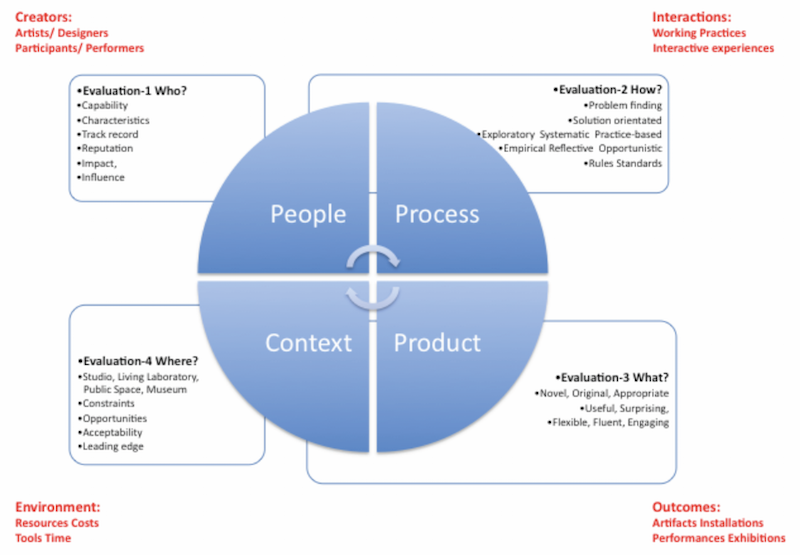
\includegraphics[width=\linewidth]{images/candy02.png}
\caption[Multi-dimensional Model of Creativity and Evaluation]{Candy's Multi-dimensional Model of Creativity and Evaluation}
\label{fig:candy02}
\end{figure}

\begin{figure}[htb] % (here, top, bottom, page)
  \centering
  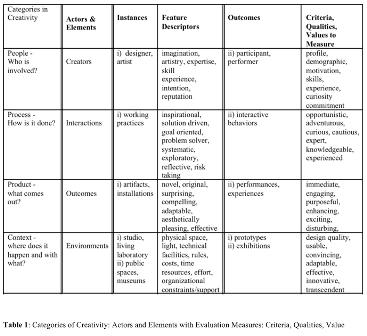
\includegraphics[width=\linewidth]{images/candy01.png}
\caption[Text for Table of Contents]{Caption text under figure}
\label{fig:candy01}
\end{figure}

\textbf{PEOPLE AS CREATORS}: \parencite[p.14-15]{Candy2012}

Criteria for evaluating creator capability:
\begin{enumerate}
  \item The creator must be able to demonstrate an ability to create an artistic outcome where subject matter, ideas and technique are combined well to produce a coherent outcome.
  \item The creator must be able to demonstrate an ability to make work that is exploratory, creative and imaginative. Interesting ideas are presented in intelligent and surprising ways.
  \item In respect of Composition and Interpretation, the creator must be able to demonstrate the ability to:\\
  •	Select subject matter that is appropriate to a given theme\\
  •	Manipulate ideas and techniques in a coherent manner\\
  •	Express ideas visually (visual communication)\\
  •	Respond in an individual and personal way
\end{enumerate}

\textbf{PROCESS AS INTERACTION}: \parencite[p.17]{Candy2012}

Criteria for evaluation can be expressed as follows
1. For a work to be deemed engaging, the participant should exhibit observable responses. There are likely to be different levels of engagement depending on whether or not the audience has had prior experience of this kind of artwork or installation or similar.\\
2. The participant responses demonstrate active engagement in three ways: Immediate, Sustained or Creative. The categories are defined as follows:\\
•	Immediate engagement: the work grabs immediate attention and yet is not so mundane as to create boredom.\\
•	Sustained engagement: the work must excite curiosity in the and also be accessible to a general audience.\\
•	Creative engagement: the work must excite immediate attention and encourage an audience to interact with it in a playful/purposeful way. As attention declines with familiarity and time, changes take place in the work that renew audience engagement.

\textbf{PRODUCT AS OUTCOME}: \parencite[p.18]{Candy2012}

Typical features for judging artworks include composition, aesthetic, affect, content, and technique. Criteria for evaluation can be expressed as follows:

•	the composition of work should be coherent, exhibit shape and balance between order and complexity.\\
•	the work should exhibit outstanding visual and sound qualities in color, line and form.\\
•	the work should be pleasing, challenging, exciting, original etc.\\
•	the content should be appropriate and effective for the chosen subject matter\\
•	the execution should demonstrate high quality technique that fits the form.

It is interesting, therefore, to consider how criteria for judging the digital arts are specified by the Prix Ars Electronica, an international competition for Cyber Arts and the foremost event of its kind today.

Entries are judged by a Jury of experts in the order of their arrival and according to the following categories:

•	Aesthetics • Originality\\
•	Excellence of execution\\
•	Compelling conception\\
•	Innovation in technique of the presentation

\textbf{CONTEXT AS ENVIRONMENT}: \parencite[p.21]{Candy2012}

Establishing a workable living laboratory for interactive art and evaluation involved setting down acceptance criteria for assessing whether or not a new interactive art system was ready to be deployed.

These included:
•	degree of robu\\stness of the art system in expectation of heavy public use
•	appropriate accessibility in respect of type of audience (e.g.\ children)\\
•	adherence to safety and house rules required by the museum\\
•	impact of other coinciding exhibits (sound, noise, light impacts)\\
•	attention to participant orientation and training\\
•	attention to art system maintenance by creator and technical support

\begin{quote}
  ``we need to apply strategies for generating clear and unambiguous data that can be turned into meaningful information. From meaningful information, we can then derive understandings related to the context of use, the outcome of which might take the form of a coherent model.'' \parencite[p.21]{Candy2012}
\end{quote}

\begin{quote}
  ``Observation as a method for data collection raises issues as to its reliability in creativity evaluation. Data from observing creativity depends upon the interpretation of what the individual observer sees.'' \parencite[p.22]{Candy2012}
\end{quote}

\begin{quote}
  ``However, in order to ‘measure’ creativity, we have to conduct research outside of controlled laboratory conditions, and cannot rely on fixed criteria that can be applied to all cases. The shifting ground and the ever-changing contexts often renders consistency out of reach.'' \parencite[p.22]{Candy2012}
\end{quote}

\begin{quote}
  ``If the term `measurement' does not match what we are doing within the creativity domain, then why do we still use this word?'' \parencite[p.22]{Candy2012}
\end{quote}

\begin{quote}
  ``Whether an action is successful or unsuccessful depends on whether the intended result is achieved.'' \parencite[p.23]{Candy2012}
\end{quote}

\begin{quote}
  ``Measuring success is more likely to be dependent on factors such as whether or not the system has engaged the audience in a playful or immersive way or whether it has elicited curiosity or excitement or concentrated attention and so on.'' \parencite[p.23]{Candy2012}
\end{quote}


% -----------------------------

% \begin{fcom}
% •	Brain operations per sec 1016 \autocite[p.194]{Kurzweil2013}\\
% •	Japan’s K-computer has 1016 calculations per sec (10 petaflops)\\
% •	Blue brain project: 2023: 1017 bytes memory + 1018 flops \autocite[p.125]{Kurzweil2013}
% \end{fcom}
%
% Human Brain Project: \autocite{Walker2012}
%
% Our brain consumes about 30W, the same as an electric light bulb, thousands of times less than a small supercomputer. \autocite[p.17]{Walker2012}
%
% For environmental and business reasons, vendors have set themselves the goal of containing energy consumption to a maximum of 20 megawatts  \autocite[p.41]{Walker2012}
%
% the 1 PFlop machine at the Jülich Supercomputing Centre could simulate up to 100 million neurons – roughly the number found in the mouse brain. \autocite[p.41]{Walker2012}
%
% Cellular-level simulation of the 100 billion neurons of the human brain will require compute power at the exascale (1018 flops). \autocite[p.41-42]{Walker2012}
%
% 2017 petascale 50petabytes memory + 50 petaflops + <=4MW power
%
% 2021 exascale 200petabyte memory + 1exaflop
%
% A second, equally important goal will be to prepare the procurement of the HBP Pre-exascale-supercomputer. By 2017/18, Jülich plans to procure a Big Data-centred system with at least 50 PBytes of hierarchical storage-class memory, a peak capability of at least 50 PFlop/s and a power consumption <= 4 MW. The memory and computational speed of the machine will be sufficient to simulate a realistic mouse brain and to develop first-draft models of the human brain. (The rest of the hardware roadmap targets an exascale machine in 2021/2022 with a capability of 1 EFlop/s and a hierarchical storage-class memory of 200 PB).\footnote{https://www.humanbrainproject.eu/high-performance-computing-platform}
%
% Chris Chatham: 10 Important Differences Between Brains and Computers \footnote{http://scienceblogs.com/developingintelligence/2007/03/27/why-the-brain-is-not-like-a-co/}
%
% \begin{enumerate}
% \item Brains are analogue; computers are digital
% \item The brain uses content-addressable memory
% \item The brain is a massively parallel machine computers are modular and serial
% \item Processing speed is not fixed in the brain; there is no system clock
% \item Short-term memory is not like RAM
% \item No hardware/software distinction can be made with respect to the brain or mind
% \item Synapses are far more complex than electrical logic gates
% \item Unlike computers, processing and memory are performed by the same components in the brain
% \item The brain is a self-organising system
% \item Brains have bodies
% \item	The brain is much, much bigger than any [current] computer
% \end{enumerate}
%
% Why Minds Are Not Like Computers \autocite{Schulman2009}
% Software – Hardware == Mind – Brain ??? analogy
%
% "The power of the computer derives not from its ability to perform complex operations, but from its ability to perform many simple operations very quickly."
%
% Layers of abstraction in computers:\\
% 1.	user interface\\
% 2.	high level programming language\\
% 3.	machine language\\
% 4.	proessor microarchitecture\\
% 5.	Boolean logic gates\\
% 6.	transistors\\
%
% layers of abstraction in brain:\\
% 1.	personality?\\
% 2.	Thinking?\\
% 3.	Chemical /electrical signals/activity?\\
% 4.	Divided Brain regions/structure\\
% 5.	Neurons\\
% 6.	Dendrites (input) and axons (output)?\\
%
%
% Computers are faster and better than humans in many tasks already.
%
% \begin{quote}
% "The weaknesses of the computational approach include its assumption that cognition can be reduced to mathematics and the difficulty of including noncognitive factors in creativity." \autocite[p.457]{Mayer1999}
% \end{quote}
%
% \subsection{Other}
%
% \begin{quote}
% "Currently many implementors of creative systems follow a creative-practitioner-type approach: produce a system then present it to others, whose critical reaction determines its worth as a creative entity. A creative practitioner’s primary aim, however, is to produce creative work, rather than to critically investigate creativity; in general this investigative aim is important in computational creativity research." \autocite{Jordanous2011}
% \end{quote}
%
% purpose or intention shifts into focus here over production of products.
%
% \begin{quote}
% "Also, evaluation of novelty (or originality, newness) is often examined in the papers cited above according to how dissimilar the system’s artefacts are to previous output or other existing examples of creative output in that domain. On the other hand, appropriateness is often evaluated according to how similar the system’s output artefacts are to known examples. Hence across the field as a whole, there is a stark inconsistency as to whether to prioritise the generation of artefacts which are dissimilar from existing artefacts, or whether to pursue the generation of artefacts which are similar to existing artefacts, arising directly from the adoption of ‘novelty + value’ as the underlying model of creativity. Such a contradiction is clearly not helping the identification of coherent and consistent strategies to adopt across the field." \autocite{Jordanous2012}
% \end{quote}
%
% \begin{quote}
% "In some cases, evaluative tests are conducted on the system which purportedly evaluate the system’s creativity but which actually only measure the system’s quality." \autocite{Jordanous2012}
% \end{quote}
%
% But if quality is the "conformance to specifications" and the specification suggested creativity, then a good quality rating of a system would automatically mean it's creative, right?
%
% \begin{quote}
% "The key conclusion of the survey was that evaluation of computational creativity is not being performed in a scientifically rigorous manner:
% \begin{itemize}
% \item The creativity of a third of the 75 ‘creative’ systems was not critically discussed.
% \item Half the papers surveyed did not contain a section on evaluation.
% \item Only a third of systems presented as creative were actually evaluated on how creative they are.
% \item A third of papers did not clearly state or define criteria that their system should be evaluated by.
% \item Less than a quarter of systems applied existing creativity evaluation methodologies.
% \item Occurrences of evaluation by people outside the system implementation team were rare.
% \item Few systems were comparatively evaluated, to see if the presented system outperforms existing systems (a useful measurement of research progress).
% \item General principles of scientific method are not being followed by the community as a whole." \autocite{Jordanous2012}
% \end{itemize}
% \end{quote}
%
% \begin{quote}
% "Reducing creativity to problem solving works when the creator is searching for an ideal solution which is not obvious, or if there is no single ideal solution but several candidates for a reasonable solution (Boden, 1994b)." \autocite{Jordanous2012}
% \end{quote}
%
% \begin{quote}
% "One potential problem with Boden’s three views of creativity is that they all assume the existence of a conceptual space, or constrained set of possibilities, that the creative individual consciously reasons with in order to be creative." \autocite{Jordanous2012}
% \end{quote}

\stopcontents[chapters]
